\section{Deep Learning Algorithm}
\subsection{Convolutional Neural Networks}
%% Why Convolutional Neural Networks (and not Naive Bayes)
Since our project deals with image classification, a deep learning algorithm was chosen, namely convolutional neural networks (CNN) as it is the state-of-the-art approach.\cite{szegedy2015going} Consequently, there are extensive libraries to utilize in this matter. In this research, the Keras library is used for the CNN in this paper.\\
A CNN takes raw image data as an input in the form of a multidimensional array. Each pixel represents a feature, possibly in several channels as it is a colored image (i.e. RGB) or a single channel as it is a grayscale image. Eventually, through training neurons by adapting weights and biases as an ordinary neural network does, class scores are received as an output. For a deeper understanding of the subject, see \cite{bloem2020deeplearning1}, \cite{karpathy2016convolutional}, on which our baseline code is based on. However, we included several conceptual changes as described later in this chapter.

\begin{figure}[h]
  \centering
  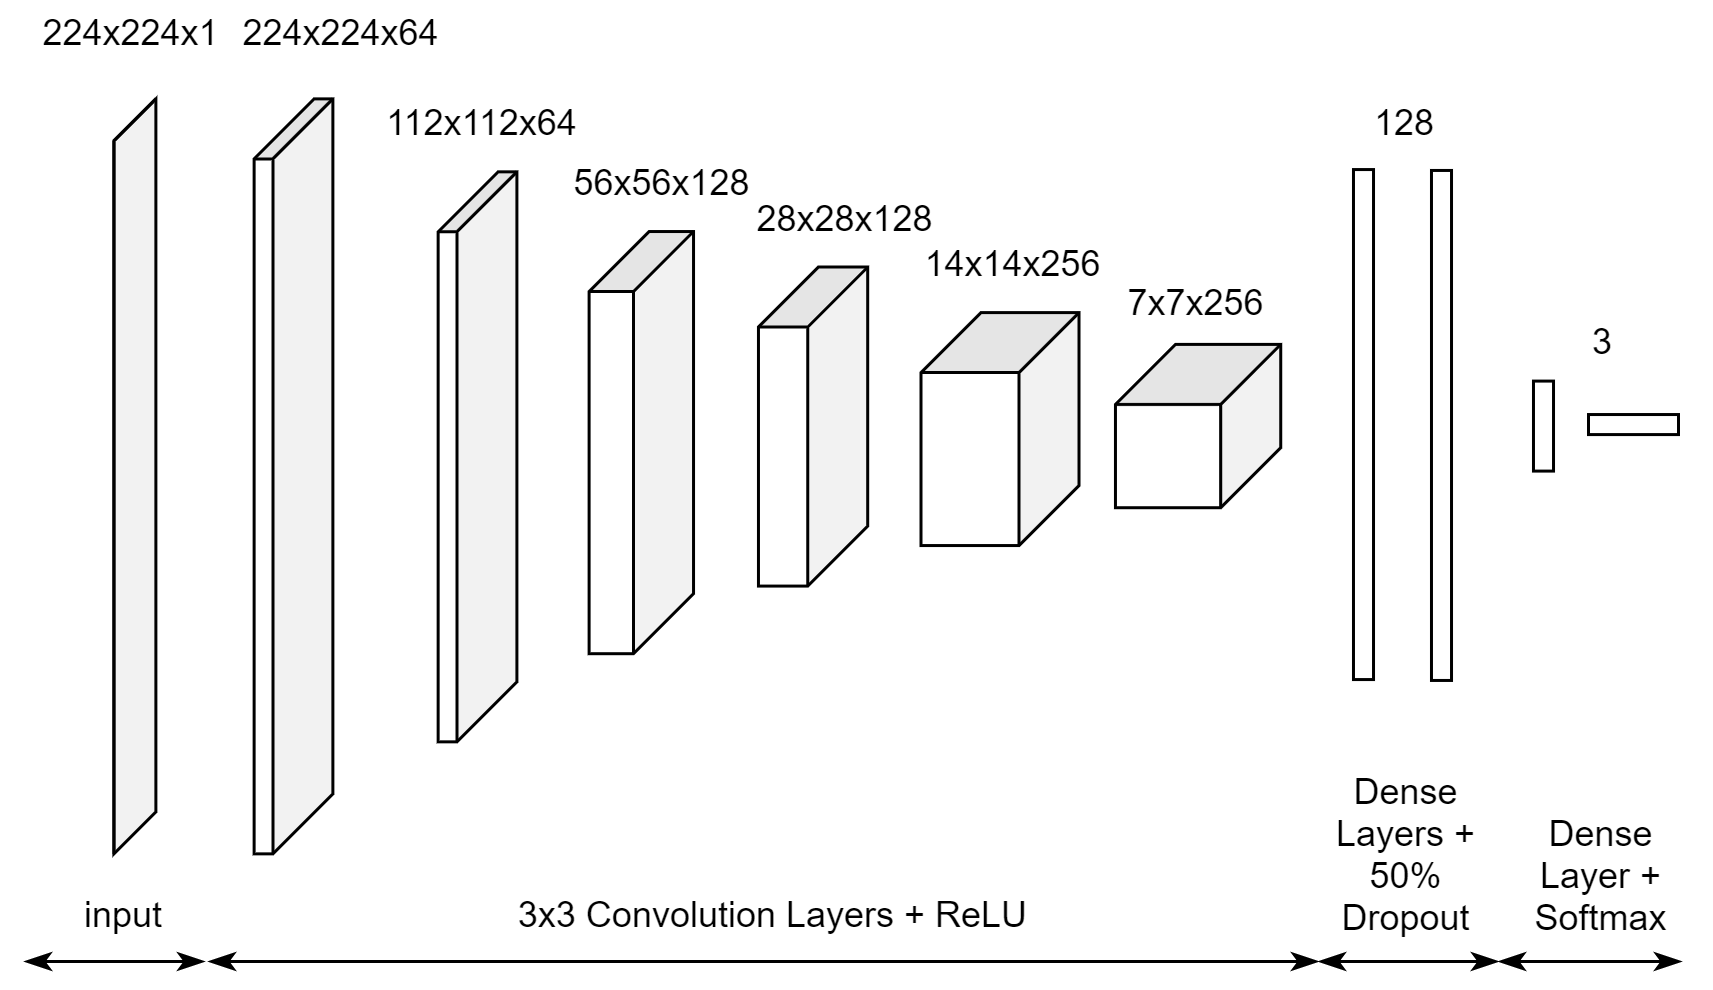
\includegraphics[width=\linewidth]{figures/cnn.png}
  \caption{schematic of the CNN used in this research}
\end{figure}

\subsection{Pre-Preprocessing}
%% Pre-Preprocessing: greyscale + Standardizing the images (224x224)
Our research discusses the influence of pre-processing measures to reduce class imbalance. To be able to compare the impact of those measures we define our raw data set not as given in Kaggle, but after some preceding preprocessing.\\
First, we change the classes from "Normal" and "Pneumonia" to "Normal", "Bacteria" and "Virus". \\
Second, we leave the separated test data as it is. We include the given validation set, as we consider it too small, to our training set, just to conduct a random 30\% split to separate the validation from the training data. According to \cite{bloem2020deeplearning1} it is considered best to have a validation set roughly the same size of the training set. Eventually, we choose a 30\% split, so that the now fixed validation set is also in a proper relation to even a smaller data set like the one prepared for undersampling.\\
Moreover, we standardize the data with $resize$ to 224x224 pixel images, which is a common number for input data \cite{karpathy2016convolutional}. Despite missing expertise in the field of pneumonia, we feel that this rescale preserves enough information while minimizing required memory and therefore speeding up the model fitting.\\
To slim down our model even further by reducing the channels from RGB to grayscale. The x-rays are already black and white, so this information is definitely abundant.\\
Eventually, this data will undergo additional preprocessing for further assessment dealing with class imbalance, which is described corresponding chapters on dealing with class imbalance.\\

\subsection{Model Fitting}
%% Strides vs Maxpooling
Based on the work of Springenberg et al. we refrain from pooling our data after every second convolution (with a single stride) as suggested in \cite{bloem2020deeplearning1}, \cite{karpathy2016convolutional}. As stated in \cite{springenberg2014striving}, it is sufficient to double the stride without losing any accuracy. This approach is called the all-convolutional net. For a concise introduction, see \cite{becker2018}.\\
%% Convolution
We stack twelve convolutional hidden layers in total including a ReLU activation layer after each convolution resulting in decreasing the image size while increasing the kernel size after every second convolution. Adding any more convolutional layers to our model have been proven counter-productive.\\ 
%% Flatten + Dropout
After the convolution layers, we flatten our data twice with dense layers. However, we avoid fully connected layers by dropping out 50\% of the data \cite{hinton2012improving} to counter overfitting \cite{srivastava2014dropout}. \\
% Regularization
However, in figure \ref{fig:cnn_opt_a} we also see that Dropout is not enough to deal with overfitting. After 12 epochs the loss function in the validation set increases again after dropping initially. That is why we also added L2-regularization for further improvement, this drastically improves the overfitting behaviour. Comparing the regularization arguments, we choose r=0.1, as it shows the best results with our model (figure \ref{fig:cnn_opt_c}). \\
%% Batchsize + Epochs
As suggested in \cite{bloem2020deeplearning1} we train our model in mini batches to utilize both advantages of stochastic gradient descent with its ability to escape local minima and full batch with increased parallelism, while also reducing the variance with bigger batches. The batch size is restricted by the GPU memory provided by Google Colaboratory, which we used in our project. As seen in figure \ref{fig:cnn_opt_b}, increasing batch size also has a positive influence on reducing overfitting. Therefore, we choose a batch size of 128, which also marks the upper boundary recommended in \cite{bloem2020deeplearning1}.\\
In total, we train the neural network in 30 epochs since our target functions have plateaued off.
\begin{figure}[!ht]
  %\begin{minipage}{0.5\linewidth}
    \centering
    \subfloat[influence regularization]{\label{fig:cnn_opt_a}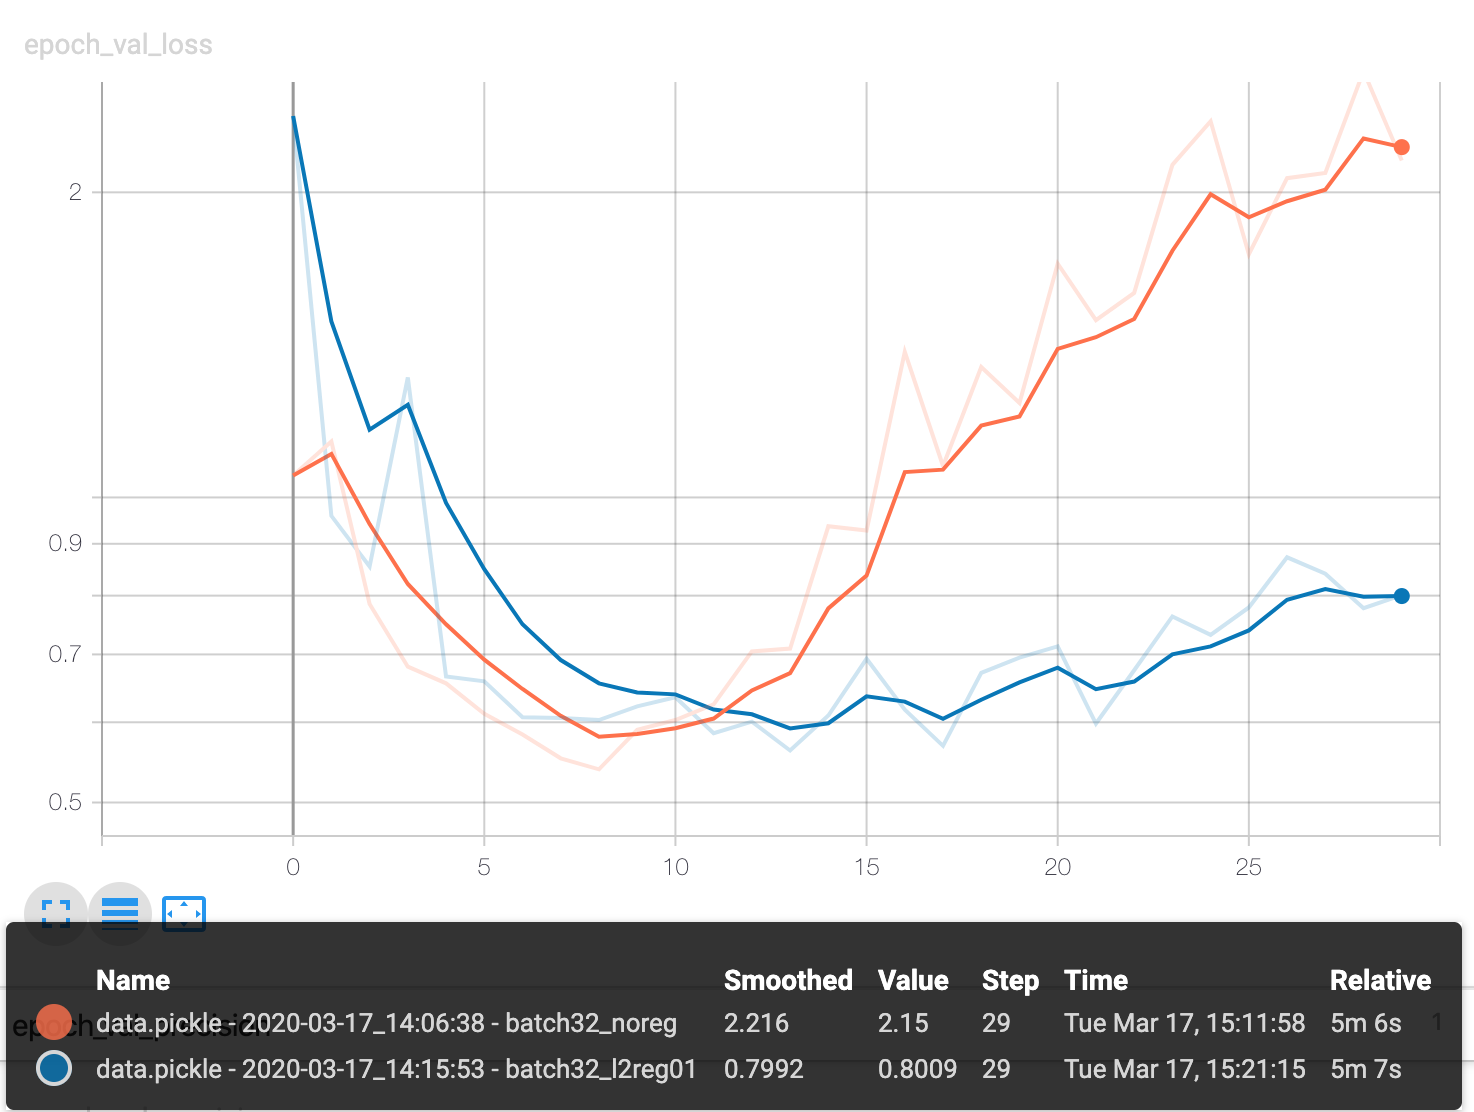
\includegraphics[width=0.89\linewidth]{figures/noregCompare.png}}
    \par\medskip
  %\end{minipage}%
  %\begin{minipage}{0.5\linewidth}
    \centering
    \subfloat[influence batchsize]{\label{fig:cnn_opt_b}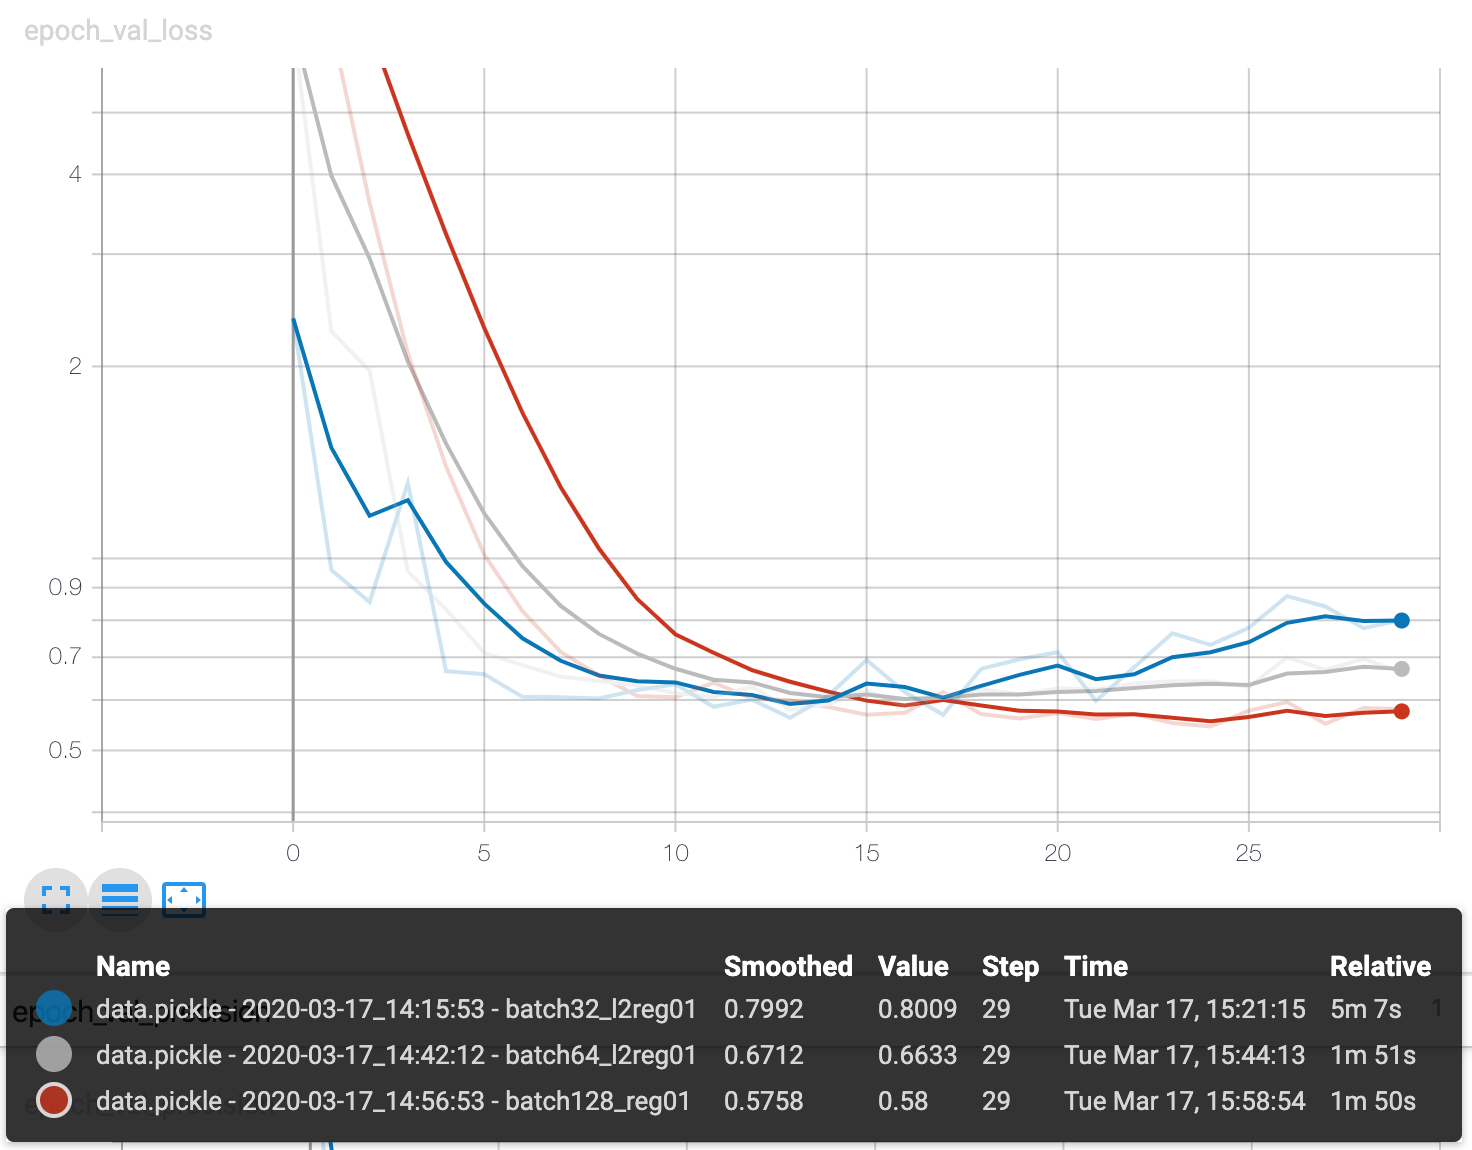
\includegraphics[width=0.89\linewidth]{figures/batchCompare.png}}
    \par\medskip
  %\end{minipage}\par\medskip
    \centering
     \subfloat[influence regularization parameter]{\label{fig:cnn_opt_c}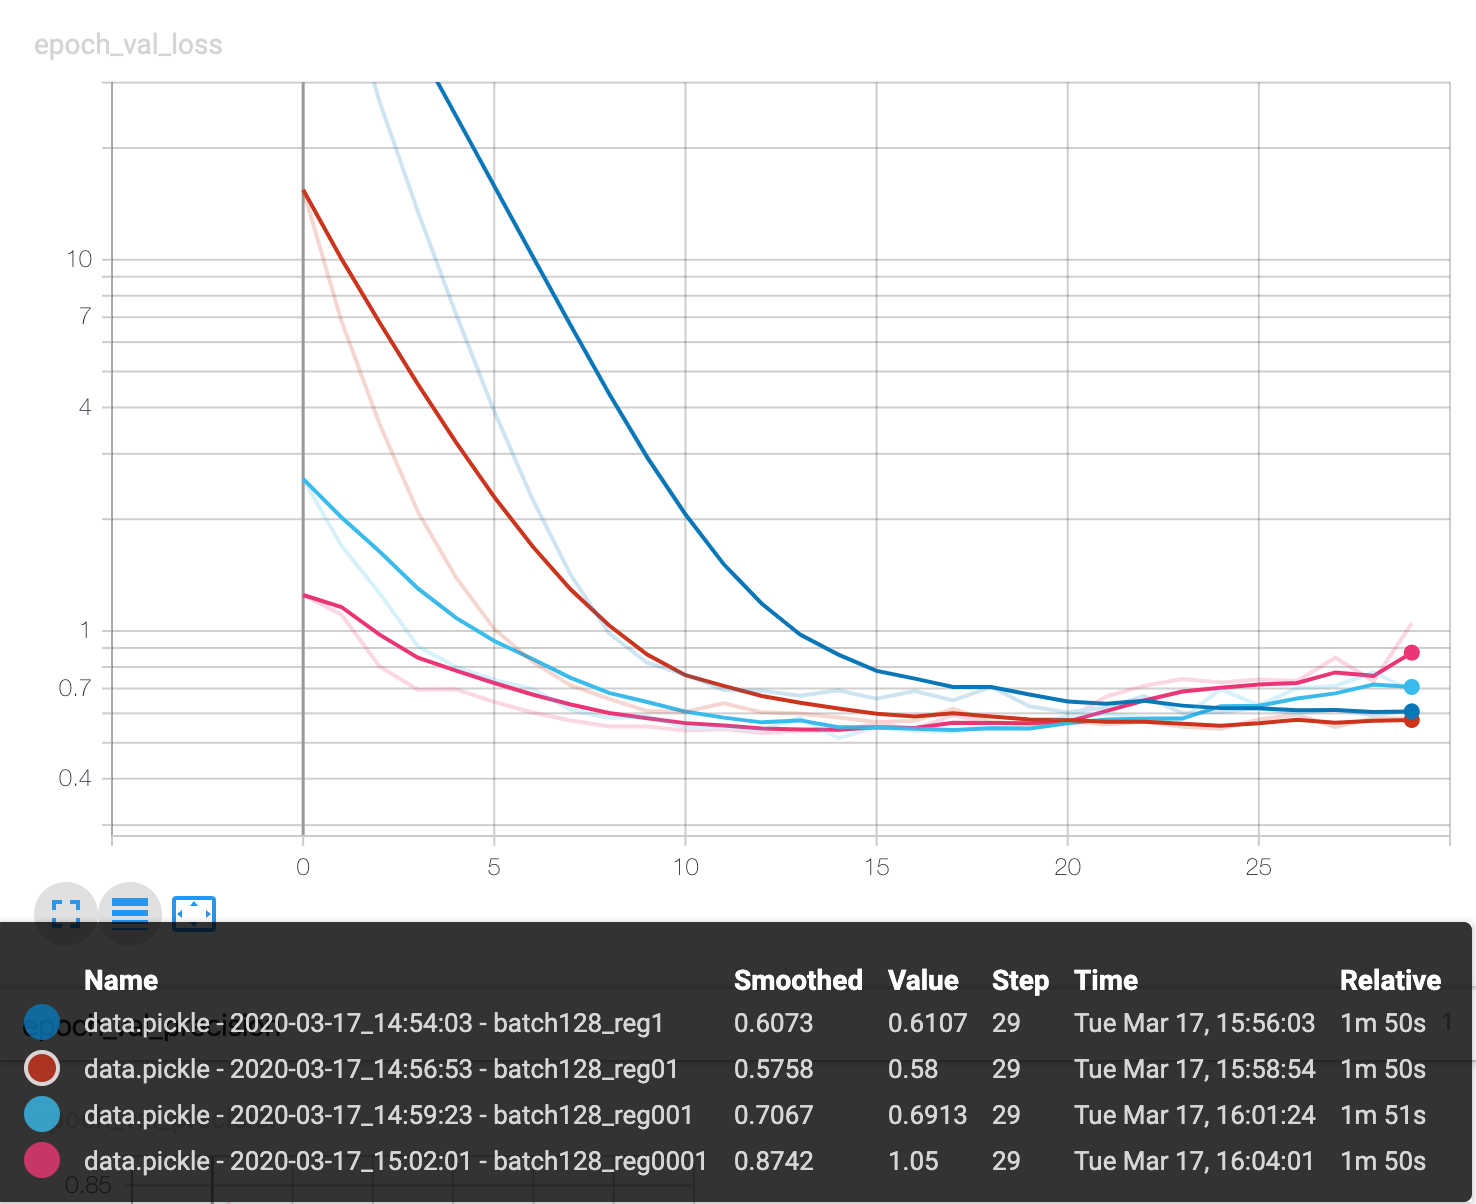
\includegraphics[width=0.89\linewidth]{figures/regCompare.png}}
    \par\medskip
  \caption{Optimizing the CNN algorithm}
  \label{fig:opt}
\end{figure}